\documentclass[tikz,border=8pt]{standalone}
\usepackage{amsmath,amssymb}
\usetikzlibrary{arrows.meta,automata,positioning,quotes}
\begin{document}
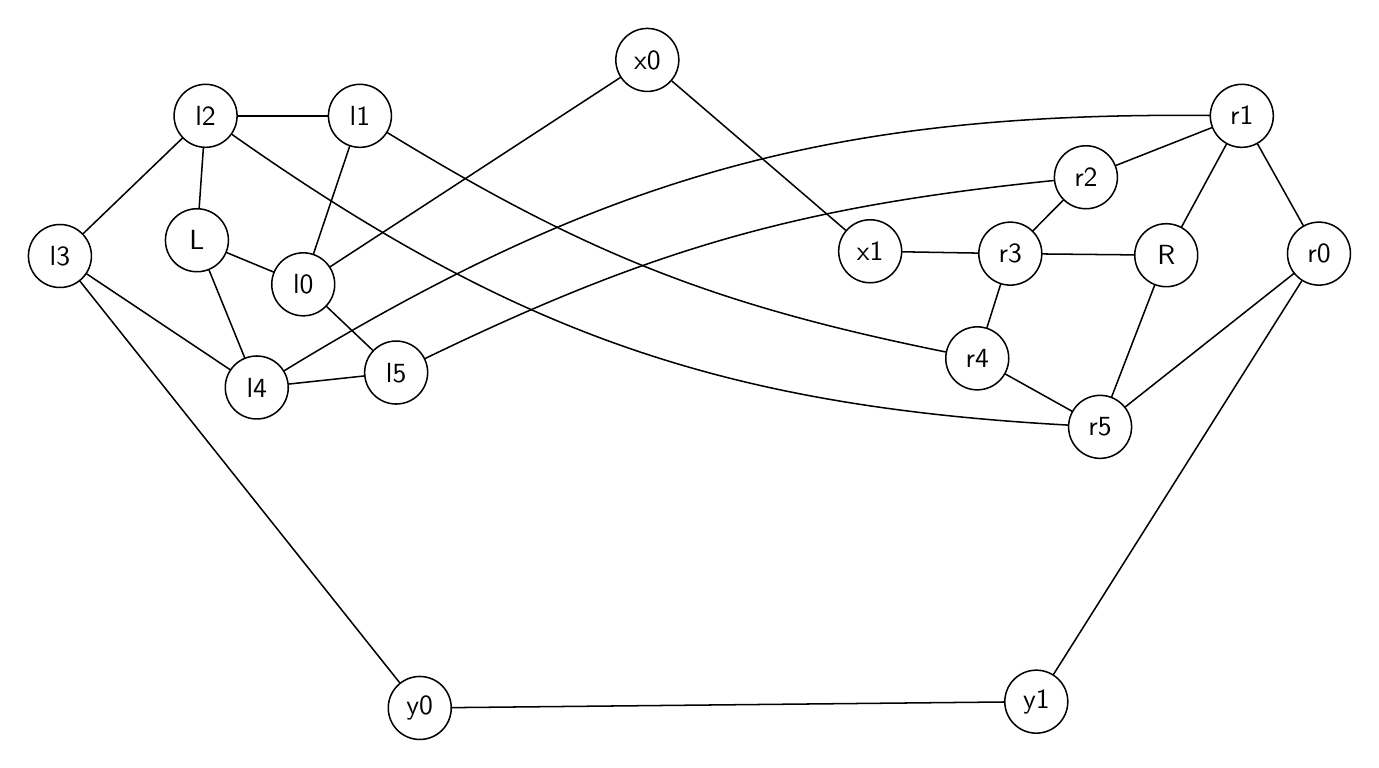
\begin{tikzpicture}[x=1cm,y=1cm]
\tikzset{
  graphnode/.style={circle,draw=black,line width=0.55pt,minimum size=8mm,inner sep=1pt,font=\sffamily},
  graphedge/.style={draw=black,line width=0.55pt,line cap=round,line join=round},
  directed/.style={graphedge,-{Stealth[length=2.4mm,width=2.0mm]}},
  undirected/.style={graphedge}
}
\node[graphnode] (n_L) at (-6.64,0.30) {L};
\node[graphnode] (n_l0) at (-5.29,-0.26) {l0};
\node[graphnode] (n_l1) at (-4.57,1.88) {l1};
\node[graphnode] (n_l2) at (-6.53,1.88) {l2};
\node[graphnode] (n_l3) at (-8.38,0.10) {l3};
\node[graphnode] (n_l4) at (-5.88,-1.57) {l4};
\node[graphnode] (n_l5) at (-4.11,-1.38) {l5};
\node[graphnode] (n_R) at (5.67,0.11) {R};
\node[graphnode] (n_r0) at (7.61,0.13) {r0};
\node[graphnode] (n_r1) at (6.63,1.88) {r1};
\node[graphnode] (n_r2) at (4.65,1.10) {r2};
\node[graphnode] (n_r3) at (3.69,0.13) {r3};
\node[graphnode] (n_r4) at (3.27,-1.20) {r4};
\node[graphnode] (n_r5) at (4.83,-2.07) {r5};
\node[graphnode] (n_x0) at (-0.92,2.59) {x0};
\node[graphnode] (n_x1) at (1.91,0.16) {x1};
\node[graphnode] (n_y0) at (-3.81,-5.64) {y0};
\node[graphnode] (n_y1) at (4.02,-5.56) {y1};
\draw[undirected] (n_l0) -- (n_l1);
\draw[undirected] (n_l1) -- (n_l2);
\draw[undirected] (n_l2) -- (n_l3);
\draw[undirected] (n_l3) -- (n_l4);
\draw[undirected] (n_l4) -- (n_l5);
\draw[undirected] (n_l5) -- (n_l0);
\draw[undirected] (n_L) -- (n_l0);
\draw[undirected] (n_L) -- (n_l2);
\draw[undirected] (n_L) -- (n_l4);
\draw[undirected] (n_r0) -- (n_r1);
\draw[undirected] (n_r1) -- (n_r2);
\draw[undirected] (n_r2) -- (n_r3);
\draw[undirected] (n_r3) -- (n_r4);
\draw[undirected] (n_r4) -- (n_r5);
\draw[undirected] (n_r5) -- (n_r0);
\draw[undirected] (n_R) -- (n_r1);
\draw[undirected] (n_R) -- (n_r3);
\draw[undirected] (n_R) -- (n_r5);
\draw[undirected] (n_l0) -- (n_x0);
\draw[undirected] (n_x0) -- (n_x1);
\draw[undirected] (n_x1) -- (n_r3);
\draw[undirected] (n_l3) -- (n_y0);
\draw[undirected] (n_y0) -- (n_y1);
\draw[undirected] (n_y1) -- (n_r0);
\draw[undirected] (n_l1) to[bend right=10] (n_r4);
\draw[undirected] (n_l2) to[bend right=16] (n_r5);
\draw[undirected] (n_l4) to[bend left=16] (n_r1);
\draw[undirected] (n_l5) to[bend left=10] (n_r2);
\end{tikzpicture}
\end{document}
